\documentclass[hyp]{socreport}

\usepackage{mathtools}
\usepackage{mathtools}
\usepackage{fullpage}
\usepackage{float}
\usepackage{hyperref}
\usepackage{graphicx}
\usepackage{amsmath}
\usepackage{caption}
\usepackage[shortlabels]{enumitem}
\usepackage[utf8]{inputenc}
\graphicspath{{./figs/}}
\DeclarePairedDelimiter{\abs}{\lvert}{\rvert}

%%% Begin document
\begin{document}
\pagenumbering{roman}
\title{Underwater Real-Time Object Recognition and Tracking for Autonomous Underwater Vehicle}
\author{Tan Soon Jin}
\projyear{2016/17}
\projnumber{H021400}
\advisor{Prof. Terrence Sim Mong Cheng}
\deliverables{
    \item Report: 1 Volume}

\maketitle

\begin{abstract}
This project proposes and implements a near real-time vision processing framework on the \textit{Bumblebee AUV (Autonomous Underwater Vehicle)} that participates in Robosub, an international autonomous robotics submarines held annually in San Diego hosted by AUVSI (Association for Unmanned Vehicle Systems International).

The implemented vision system will be deployed on the AUV to complete a series of visual tasks during the competition that mimics real world underwater application such as collecting data on marine life-forms, repairing underwater pipeline etc. Though there are many state-of-the-art vision algorithms developed by the community, the underwater domain poses an entirely different set of challenges such as low contrast, color degradation and underwater perturbations that demands a different vision processing approach.

The primary contribution of the project is to implement a vision framework consisting of a set of modular vision modules and pipelines for real-time object tracking in different underwater conditions. It is essential that the the vision framework is both a) adaptive, b) robust and c) easy to use. With the implemented vision modules, the project's secondary contribution aims to automate parameter selection and model selection; taking the human out of the loop.

\begin{descriptors}
    \item Computer System Implementation
    \item Visual Computing
\end{descriptors}
\begin{implement}
    Python, ROS (Robot Operating System)
\end{implement}
\end{abstract}

\begin{acknowledgement}
    I would like to acknowledge the advice and guidance by my supervisor Prof. Terrence Sim Mong Cheng in this project.
\end{acknowledgement}


\listoffigures
\listoftables

%%%%%%%%%%%%%%%%%%%%%%%%%%%%%%%%%%%%%%%%%%%%%%%%%%%%%%%%%%%%%%%%%%%%%%%%%%%%%%%
% Chapter 1
%%%%%%%%%%%%%%%%%%%%%%%%%%%%%%%%%%%%%%%%%%%%%%%%%%%%%%%%%%%%%%%%%%%%%%%%%%%%%%%

\chapter{Introduction}

\section{Background on Robosub}

\subsection{Information about the competition}
Robosub is an international AUV competition where students from around
the world build their own customized AUV to complete a series of
underwater missions that involve both visual tasks and acoustics task.
The competition is held annually in TRANSDEC (Transducer Evaluation
Center) man-made pool.

\begin{figure}[ht]
\centering

        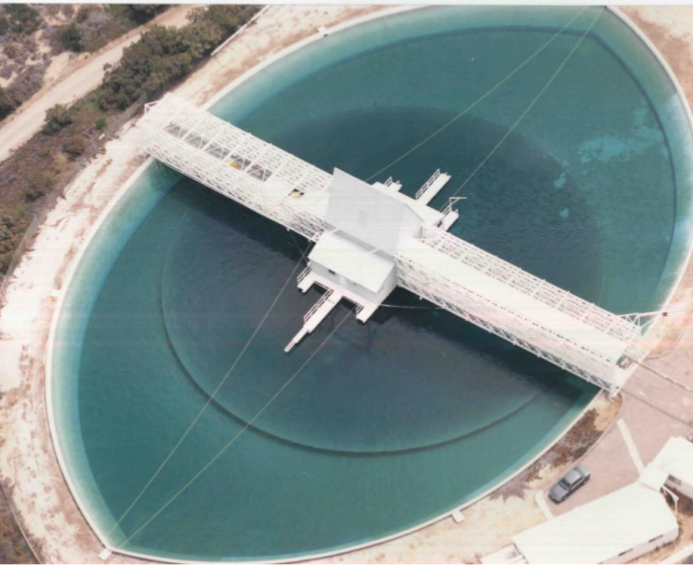
\includegraphics[width=0.8\textwidth, height=0.3\textheight]{transdec_aerial.png}
        \caption{Aerial view of TRANSDEC. Operational depth of 16 ft for most vision tasks}
        \label{fig:transdec_aerial}

\end{figure}

\subsection{Description of vision tasks}
Vision tasks in Robosub can divided into forward-facing tasks and
bottom-facing tasks which poses different sets of challenges. Since the
tasks do not vary significantly every year, we can use datasets
collected from this year's competition as testbed for our vision
algorithms.

\begin{figure}[ht]
\centering

        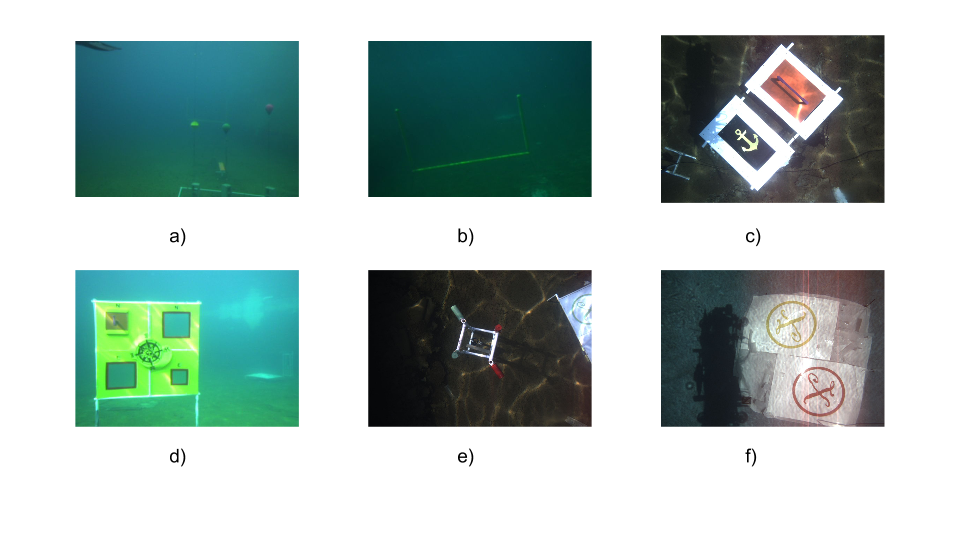
\includegraphics[width=0.8\textwidth, height=0.3\textheight]{robosub_vision_tasks.png}
        \caption{Robosub 2016 Vision Tasks. a) Scuttle Ship b) Navigate
        Channel c) Weigh Anchor d) Set Course e) Bury Treasure (Coins)
        f) Bury Treasure (Island)}
        \label{fig:robosub2016_tasks}

\end{figure}

\begin{enumerate}
    \item \textbf{Scuttle Ship (Buoy)}
        A recurring task where the AUV has identify the correct color
        buoy and touch it. There are two major challenges with this
        task:
        \begin{enumerate}[a.]
        \item Red buoy tends to exhibit color distortion as red
          wavelength attenuates the fastest \cite{Galdran2015}.
        \item Non-uniform illumination on top-half of buoys make it hard
          to distinguish the buoys.
        \end{enumerate}
    \item \textbf{Navigate Channel} \\
        The AUV is required to move in between and over the PVC pipes.
    \item \textbf{Weight Anchor} \\
        Classic object classification task where the AUV is required to
        drop a marker into the correct bin to obtain maximum points
        after removing the cover using a manipulator.
    \item \textbf{Set Course} \\
        Identification of covered square (orange panel) and remove it.
        Fire two markers over 2 smaller holes. As yellow and orange are
        really close on the colour spectrum, this forces us to use other
        visual cues such as edge for better detection.
    \item \textbf{Bury Treasure} \\
        For this task, one has to identify the small cylinders (red and
        green) and drop them onto their respective colored circles (on
        the Island). Identifying and distinguishing small objects afar
        (4 m) underwater is the biggest challenge in this task. Besides
        that, the dropped cylinders may potentially occlude the circles.
\end{enumerate}

\section{Challenges in Underwater Image Processing}

Many literature such as \outcite{M2016} that investigates various
underwater image restoration methods cite haze formation which happens
as light propagated from object undergoes attenuation and scattering
causing image with low contrast. In addition, Beer-Lambert law
\cite{gevers2012color} states relates attenuation of light to properties
of water medium; therefore, light components with low wavelength; green
and blue are not as easily absorbed compared to red wavelength. This
causes underwater images tend to have greenish or bluish color cast.

\begin{figure}[ht]
\centering

        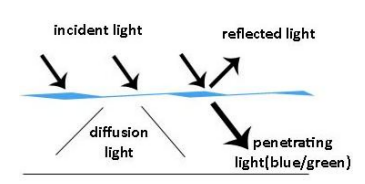
\includegraphics[width=0.8\textwidth, height=0.2\textheight]{underwater_beerlambert.png}
        \caption{Absorption of light at the surface}
        \label{fig:water_surface_effect}

\end{figure}

\section{Project Requirements Analysis}
Though it is the objective of the project to design a vision framework
for the Robosub missions, the vision framework should also be easily
extended to work for more complex real world applications. 

\subsection{Nature of tasks}
\begin{enumerate}
    \item Vision algorithms perform with acceptable accuracy under the following conditions:
    \begin{figure}[ht]
    \centering
            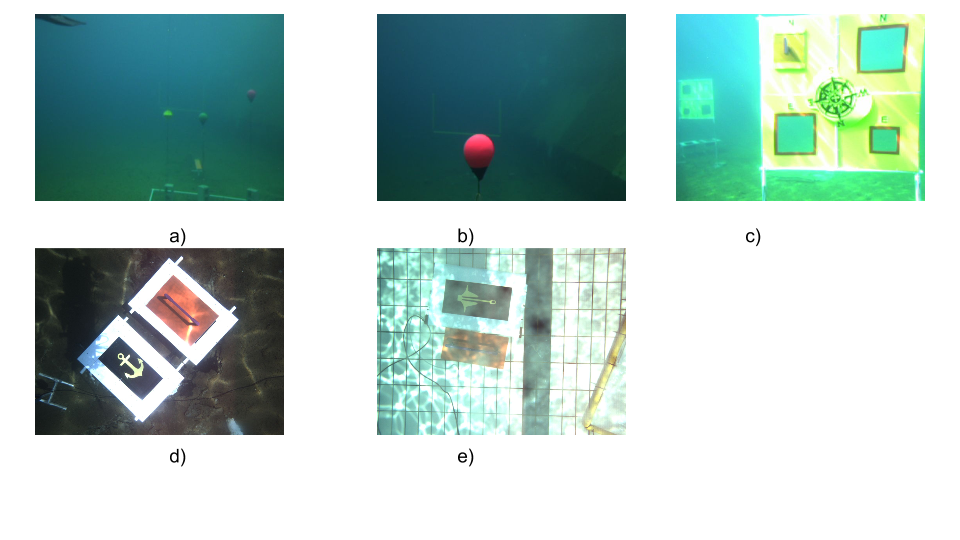
\includegraphics[width=0.8\textwidth, height=0.3\textheight]{task_challenges.png}
            \caption{Different vision challenges. a) Haze formation b)
            Partial occlusion c) Non-uniform illumination d) Sunlight
            flickers e) Shadow}
            \label{fig:vision_challenges}
    \end{figure}
    \item Low detection latency (near real-time) \\
        AUV needs to make swift decision based on sensor inputs to
        complete task under time constraints (same for real world time
        critical mission i.e underwater mine detection)
    \item Geometric properties of objects are made known in advance
    \item Short-period single target tracking for  task (unlike video surveillance application)
    \item Able to detect objects from far away (5m) and near distance (for manipulation task)
\end{enumerate}

%%%%%%%%%%%%%%%%%%%%%%%%%%%%%%%%%%%%%%%%%%%%%%%%%%%%%%%%%%%%%%%%%%%%%%%%%%%%%%%
% Chapter 2
%%%%%%%%%%%%%%%%%%%%%%%%%%%%%%%%%%%%%%%%%%%%%%%%%%%%%%%%%%%%%%%%%%%%%%%%%%%%%%%

\chapter{Literature Review}
This review is conducted with the purpose to investigate and select most
suitable algorithms that generate the best result on the Robosub
datasets. Since every teams who participate in Robosub are required to
submit a journal paper,vision algorithms deployed by top-peforming
schools such as Cornell University, University of Florida and École de
technologie supérieure provide valuable insights on image processing
that are effective in underwater environment. Besides that, review of
popular image processing techniques in particular on topics like object
detection, object tracking, color constancy, saliency mechanism,
detection proposals and adapatation of algorithms.

\section{Preprocessing}
\subsection{Underwater Image Enhancement}
The paper by \outcite{garcia2002way} compared methods such as
homomorphic filtering and local adaptive histogram equalization
(Contrast Limited Adaptive Histogram) which considers that image is a
product of illumination and reflectance properties. However, homomorphic
filter has the benefit of preserving sharp edges while attenuating
non-uniform illumination. On the other hand, by only redistributing
pixels exceeding a clipping level to increase contrast of an image,
CLAHE manages to reduce noise amplification in normal local histogram
equalization.

Instead of relying on a single image, \outcite{Gracias2008} recover
corrupted underwater image by finding the difference between the current
frame with temporal median of a registered set of N frames. Image
dehazing is equally as important to ensure good performance of further
image processing operation such feature detection. \outcite{Kaiming2011}
proposed a single image dehazing method using the dark channel prior
which states that haze-free image contains local region with low
intensities in at least one color channel. \outcite{Galdran2015} propose
a variant of dark channel prior for underwater environment, the Red
Channel method as red color shows most degradation in turbid water
medium. From another perspective, \outcite{Ancuti2011} takes a
fusion-approach to recover the original image by generating a few weight
maps that correlates with intrinsic properties of the image itself. A
color corrected and contrast enhanced of the input image are used to
generate different weight maps that are fused using a Laplacian
multi-scale strategy to generate a smoothed output image. This method
has the benefit of using a single image but the weight maps must be
combined with different weightage to achieve an ideal result. 

\subsection{Color Constancy}
Color cue plays an important role to distinguish different objects such
as the small cylinders in Robosub that requires sorting by color. The
ability to account for color of the light source is called color
constancy. The work of \outcite{Gijsenij2011} analyzes various color
constancy algorithms. Attention is paid especially on low-level
statistics methods that are computationally inexpensive compared to
learning-based methods. The Grey-World \cite{buchsbaum1980spatial}
estimate the color of the light source by estimating the average color
in the image assuming that any deviation from average color (Grey) is
caused by illuminants. The White-Patch method \cite{land1977retinex}
estimates the color of light source by computing the maximum response in
individual RGB color channels. \outcite{finlayson2004shades} shows that
both Grey-World and White-Patch algorithms are special instantiation of
a more general color constancy algorithm based on Minkowski norm called
Shades of Grey. Their investigation of best illumination estimation
suggests using Minkowski norm, p = 6 to obtain optimal performance.

Though we see new method such as the Color Rabbit \cite{Bani??2014}
which combine multiple local illumination estimations to a global one,
these class of methods are more computationally expensive which is not
suitable for real-time application. Inspired by primary visual cortex
(V1) of human visual system (HVS), \outcite{Gao2013} estimate the true
illuminant color of a scene by computing the maximum response in
separate RGB channels of the responses of double-opponent cells. This
method is shown to perform better on outdoor scenes from Gehler-Shi
dataset where the mean reflectance is not achromatic which is assumed by
Grey-World based methods. 

\section{Saliency Region Detection}
Ability of human visual system (HVS) to selectively process only the
salient visual stimuli, specifically salient object detection helps to
reduce computation time of object recognition that traditionally relies
of sliding-window approach to detect object of interest.
\outcite{achanta2009frequency} estimate centre-surround contrast using
color and luminance features using a frequency-tuned approach to
generate high-resolution saliency map. In contrast, biological inspired
method of \cite{Itti1998} that computes centre-surround contrast using
Difference of Gaussian (DoG) which generates low resolution map and
ill-defined boundaries because of down sampling of original
image.Because saliency detection often work poorly in low contrast
environment i.e underwater environment, work of
\outcite{VanDeWeijer2005} boost local color information by analyzing
isosalient colour derivatives. \outcite{Cao2010} extended work of Van de
Weijer as Gaussian derivatives of each opponent color to get a better
iso-salient transformation. 

\section{Detection Proposals}
Relying on saliency mechanism is insufficient in perturbed underwater
condition; therefore, different detection proposals algorithms are
investigated. \outcite{Hosang2015} cited that "detection proposals"
which can be grouped into a) grouping proposal methods and b) Window
scoring proposals methods are used extensively by top performing object
detectors in PASCAL and ImageNet. On top of reduced computation cost by
avoiding exhaustive sliding window approach, detection proposals improve
recall by filtering out false positives. Recent work of
\outcite{Winschel2016} combines top performing detection proposals
methods, SelectiveSearch \cite{uijlings2013selective} and EdgeBox
\cite{zitnick2014edge}. Though detection proposals allow for faster
object recognition, it is important that it does not filter out object
of interest and incur more computation costs that out weights time
saved.

\section{Object Detection and Tracking}
An overall review of journal papers submitted by top-performing teams in
Robosub shows a general trend of combining surprisingly simple computer
vision techniques such as adaptive color thresholding, edge detection
i.e Canny Edge \cite{canny1986computational}, and contour analysis i.e
Hu moment \cite{hu1962visual}. Team CUAUV (Cornell AUV) proposes
adaptive color thresholding on different color spaces such as LAB, LUV
and YCrCb where the individual masks are combined to form final
binarized mask. This is a blob-based detection approach where contour
generated by OpenCV's implementation of  \cite{suzuki1985topological}
will be matched against known geometric properties of desired object of
interest. \outcite{Walters2014} use particle filter approach to detect
and track object of interest. Known for its ability to deal with
non-linear noise and multi-modal hypotheses
\cite{isard1998condensation}, particle filter has the ability to recover
from wrongly tracked objects. Though more sophisticated techniques such
as neural-network classification is deployed, teams still generally rely
on low-level visual cues such as color and edge. This may be attributed
to simplicity and efficiency of mentioned algorithms.
\outcite{Benoit2014} focuses on developing sophisticated vision tuning
client that allows for rapid prototyping via "mix and match" approach to
design a suitable vision pipeline for each individual vision tasks.

%%%%%%%%%%%%%%%%%%%%%%%%%%%%%%%%%%%%%%%%%%%%%%%%%%%%%%%%%%%%%%%%%%%%%%%%%%%%%%%
% Chapter 3: Design & Methodology
%%%%%%%%%%%%%%%%%%%%%%%%%%%%%%%%%%%%%%%%%%%%%%%%%%%%%%%%%%%%%%%%%%%%%%%%%%%%%%%

\chapter{Design \& Methodology}

\section{Proposed design}

Though many solutions to underwater vision challenges exist, many of them are
not designed to work with each other as they do not share a common interface. To
increase ease of use and productivity of developers, this paper proposed a
vision framework that consists of modular components tailored for underwater
application, and ease of integration to Robot Operating System (ROS) which are
commonly used by the robotics community.

The proposed vision framework is divided into \textit{offline} modules and
\textit{online} modules. \textit{Offline} modules refer to modules that will
deployed prior to object tracking mission such as video annotation, visual data
analysis and model learning. In contrast, \textit{Online} modules are deployed
during mission such as preprocessing, object detection and object tracking.

\begin{figure}[H]
\centering
  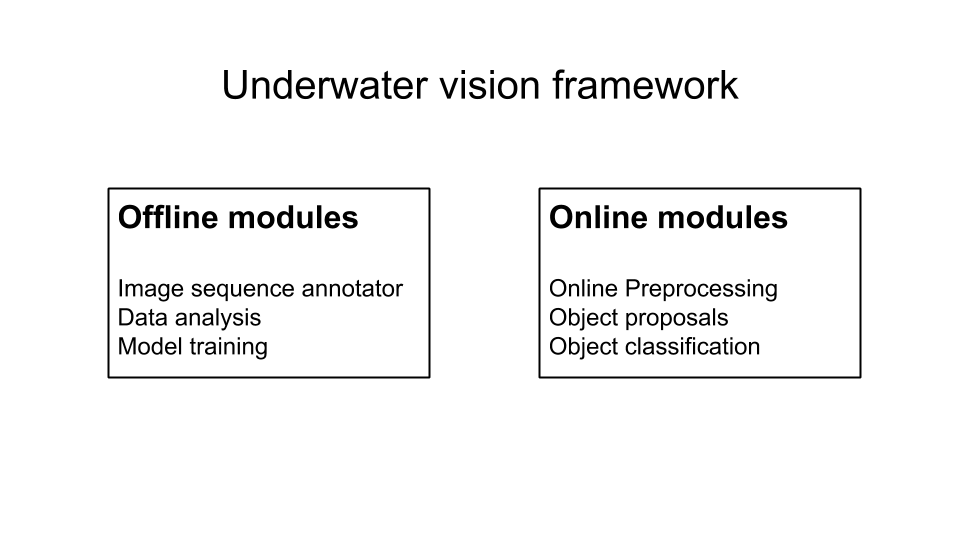
\includegraphics[width=0.8\textwidth, height=0.3\textheight]{framework.png}
  \caption{Proposed vision framework}
  \label{fig:proposed_vision_framework}
\end{figure}

\subsection{Offline modules}

\textbf{Video annotation} is extremely important for ground truth
generation that is essential for model learning. To achieve rapid ground truth
generation with limited manpower and time, model-free tracking method such as
mean-shift by (\outcite{comaniciu2002mean}) and correlation-filter based tracking
(\outcite{bolme2010visual}). Of course this is under the assumption that some
degree of localization error is acceptable and human intervention is used to
redefine the target window if drift occurs. This enables a faster testing
iteration as data collected can be integrated more quickly to update our model.

\textbf{Data analysis} helps us discover patterns and statistical nature of
collected visual data which is important for feature engineering and model
learning. These tools include visualization of image under different color
spaces, estimation of illuminants, saliency map generation and image quality
assessments. This information is used as metadata to label and categorize
dataset to increase productivity of model training and validation. Again, this
is an attempt to automate trivial task that require human attention.

\textbf{Model Training} is divided into several stages such as feature
selection, model selection and hyperparameters optimization. To increase
usability of the software without machine learning knowledge, this paper adopt the trending
automatic machine learning approach by leveraging on available open-source
libraries such as \href{https://github.com/automl/auto-sklearn}{Auto-Sklearn},
\href{https://github.com/rhiever/tpot}{TPOT}, and \href{https://github.com/automl/HPOlib}{HPOlib}.

\subsection{Online modules}

\textbf{Preprocessing} has considerable effect on accuracy of underwater object
detection because of the challenges mentioned. Color normalization is performed
on image to remove effect of color cast because of light attenuation. Low-level
stastical methods have been explored because they are simple to implement and
fast while producing accuracy comparable to other methods such as gamut mapping
and learning methods \outcite{Gijsenij2011}. In addition, fusion-based
underwater image enhancement by \outcite{fang2013effective} is implemented to
remove haze effect because of back-scattering of light. Following that, various
illumination compensation methods are executed to reduce effect of flickering and
adjusting brightness of the image for more optimal object detection.

\textbf{Object Tracking} is separated into 3 components: a) \textit{object
  proposal}, b) \textit{object classification} and c) \textit{online preprocessing}. An
adaptive object model and pre-learned object model are applied to achieve higher
tracking accuracy. \textit{Object proposals} based on superpixel, edge-detection
and saliency are exploited to produce candidates for classification instead of
the traditional sliding-window approach which is more computationally expensive.
For \textit{object classification} of candidate windows, Support Vector Machine
(SVM), Random Forest and Gaussian Process are the supported classifiers.
To improve generalization of the tracker to different conditions,
\textit{preprocessing} steps are taken to ensure invariance to non-uniform
illuminations and underwater challenges.

\newpage
\section{Methodology}

In this section we will explain how these modular components are used together
for underwater real-time object tracking.

\begin{figure}[H]
\centering
  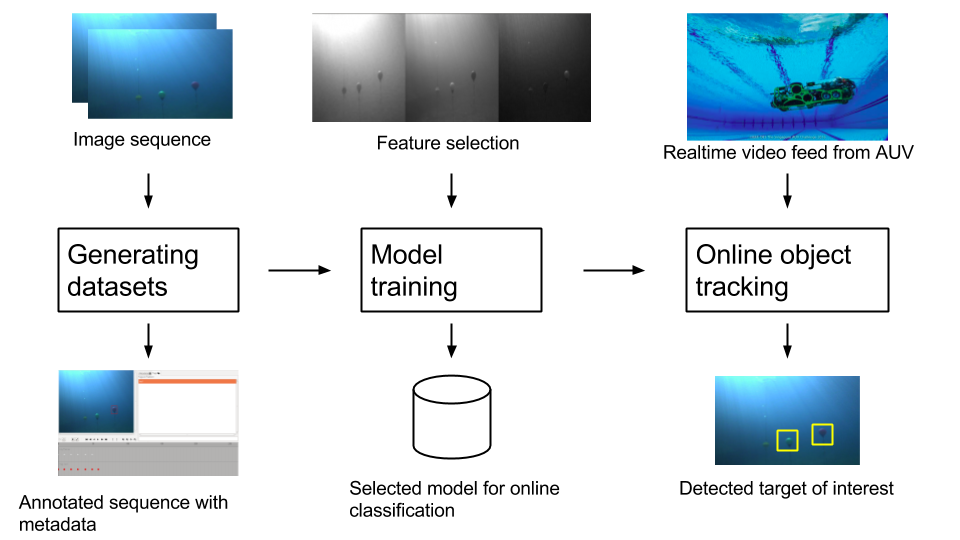
\includegraphics[width=0.8\textwidth, height=0.3\textheight]{method.png}
  \caption{Main methodology}
  \label{fig:main_methodology}
\end{figure}

\subsection{Generating datasets}

\begin{figure}[H]
\centering
  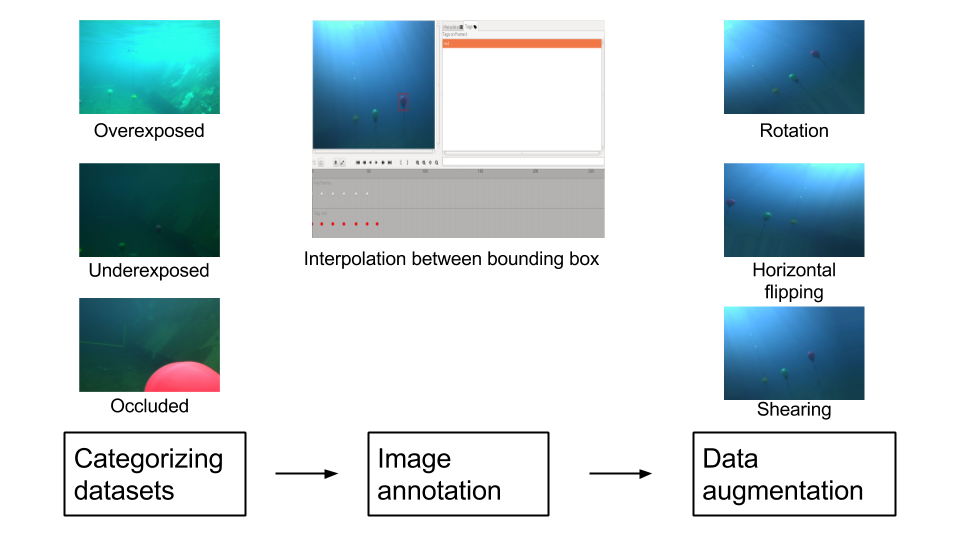
\includegraphics[width=0.8\textwidth, height=0.3\textheight]{dataset_method.png}
  \caption{Dataset generation methodology}
  \label{fig:dataset_methodology}
\end{figure}

\textbf{Data analysis} is performed on all images to further categorize them into
different datasets according to various criteria such degree of haze, existence
of shadow, illuminations and color cast. Each dataset will be tagged with
metadata generated from the analysis. Next, \textbf{video annotation} is
conducted using \textit{Mean-Shift} tracker on preprocessed images to generate
ground truth that will be used for training and validation. To prevent
overfitting and help the model generalize better, data augmentation via
horizontal flipping, scaling, rotating, shifting and color jittering is
performed with the aid of \href{https://keras.io/preprocessing/image/}{Keras
  preprocessing module}.

\subsection{Model Learning}

\begin{figure}[H]
\centering
  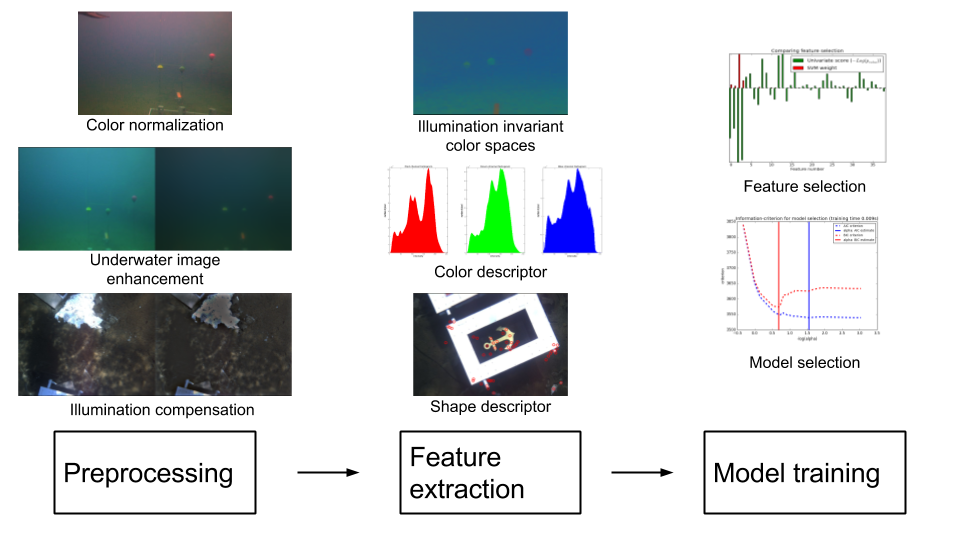
\includegraphics[width=0.8\textwidth, height=0.3\textheight]{training_method.png}
  \caption{Model learning methodology}
  \label{fig:training_methodology}
\end{figure}

To improve discriminability of objects from background in undewater setting,
\textbf{preprocessing} steps are taken such as color normalization, illumination
compensation and image enhancement. Moving on, different type of features are
extracted from various color spaces that will be used in object classification.
Using the validation set, \textbf{feature selection}, \textbf{model selection}
and \textbf{hyperparameters optimization} are executed to determine the most
optimal combination of algorithm-parameters pair for a particular object class.

\subsection{Online object detection and tracking}

\begin{figure}[H]
\centering
  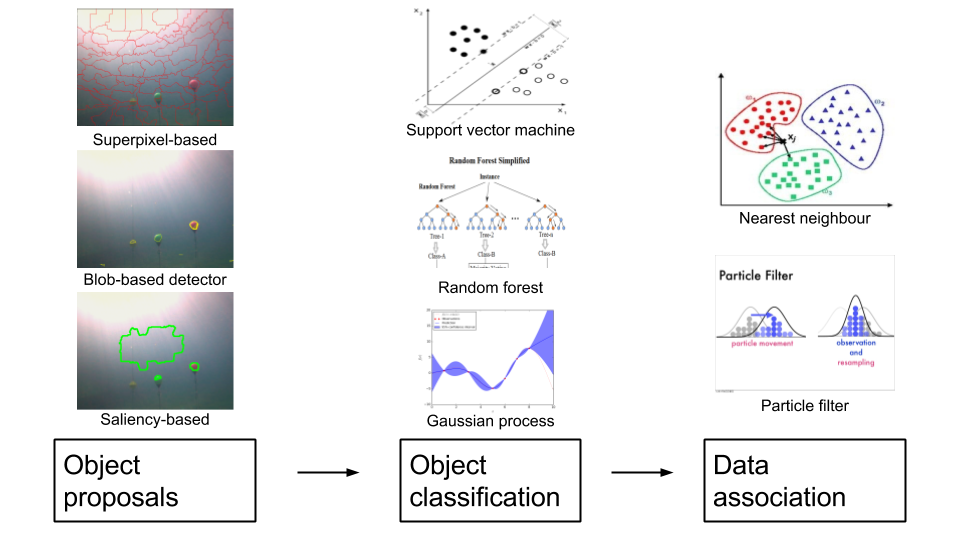
\includegraphics[width=0.8\textwidth, height=0.3\textheight]{tracking_method.png}
  \caption{Object tracking methodology}
  \label{fig:tracking_methodology}
\end{figure}

The next phase involves real-time \textbf{object proposals} adopting a)
superpixel-based clustering and b) edge detection. \textbf{Object classifier}
will rank these candidates according to classfication score. Tracking is
performed using a simple nearest neigbour approach and a new tracker will be
initialized after losing track of the target for 10 frames.

%%%%%%%%%%%%%%%%%%%%%%%%%%%%%%%%%%%%%%%%%%%%%%%%%%%%%%%%%%%%%%%%%%%%%%%%%%%%%%%
% Chapter 4: Preprocessing
%%%%%%%%%%%%%%%%%%%%%%%%%%%%%%%%%%%%%%%%%%%%%%%%%%%%%%%%%%%%%%%%%%%%%%%%%%%%%%%

\chapter{Preprocessing}

In this section, we will look into detail the preprocessing steps that are
applied to each image. 

\section{Color Normalization}

For underwater vision challenges, color cues are very important features because
other features like edge, texture and corner have poor visibility underwater
because of low contrast. In Robosub, there are several vision tasks that
requires classification of different objects based on their colors. Though color
cue is a simple and discriminative feature for underwater object
detection, color feature shows very poor repeatability under varying light
source. To achieve consistent feature extraction, this paper takes a
\textit{static} approach (fixed-parameters) because of simplicity and our
application does not require high degree of accuracy. With the static approach,
there are less parameters needed to be optimized.

\begin{figure}[H]
\centering
  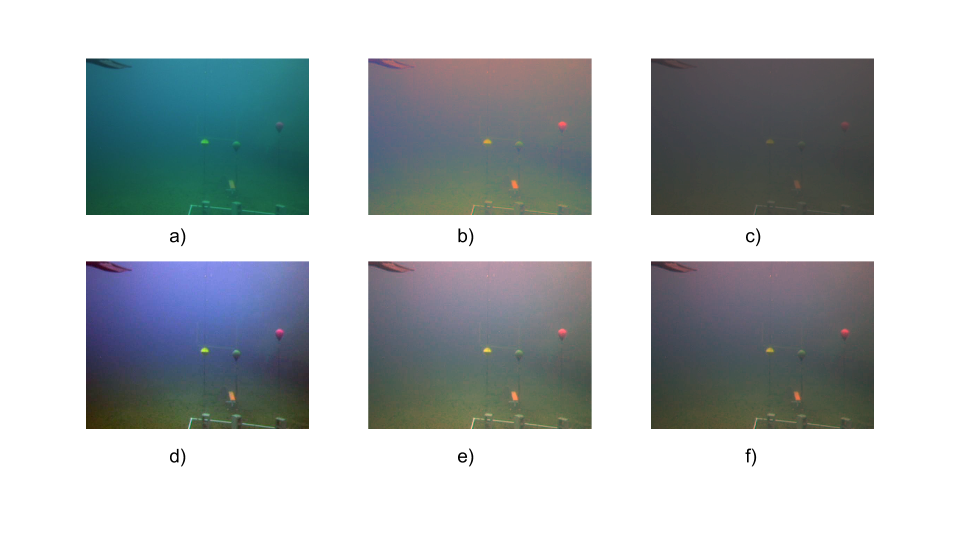
\includegraphics[width=0.8\textwidth, height=0.3\textheight]{color_constancy.png}
  \caption{Color normalization results (left to right): \newline Top row:
  a) Raw input, b) Finlayson's comprehensive normalization, c) Grey-world \newline Bottom
  row: d) IACE, e) Finlayson's non-iterative normalization f) Shade of Gray}
  \label{fig:colorconstancy_results}
\end{figure}

This paper only considers color normalization methods that require single image
without prior information about the camera used. There are 2 main steps to any
color normalization method: a) illuminant estimation and b) image correction.
The aim of image correction is to achieve chromatic adaptation which can be
modelled with a diagonal transformation \outcite{von1970influence} with certain assumptions.
The mapping of an image under unknown light source to an image under canonical
light source is performed using a diagonal matrix as shown below:

\[
\begin{pmatrix}
  R_c \\
  G_c \\
  B_c \\
\end{pmatrix}
=
\begin{pmatrix}
  d_1 & 0 & 0 \\
  0 & d_2 & 0 \\
  0 & 0 & d_3\\
\end{pmatrix}
\begin{pmatrix}
  R_u \\
  G_u \\
  B_u \\
\end{pmatrix}
\]

Results from \outcite{gijsenij2011computational} suggests that different
algorithms show their strenghts and weaknesses on different datasets. Therefore,
this paper proposes a some color normalization strategies that can be chosen
based on performance of object detection on the validation datasets.

\subsection{Algorithm Implementation}


\subsubsection{Grey-World based}

\begin{enumerate}

\item \textbf{Grey-World} \\ 
With the assumption that: \textit{the average reflectance
in a scene under a neutral light source is achromatic} \outcite{buchsbaum1980spatial}, the colour of the light
source is estimatd by computing the average color in the image.

\item \textbf{White patch} \\
With the assumption that: \textit{the maximum response of RGB channels is caused
by the perfect reflectance} \outcite{land1977retinex}, the colour of the light
source is estimatd by computing the maximum pixel value of each channel separately.

\item \textbf{Grey-Edge} \\
Instead of using raw pixel value, \outcite{van2005color} makes the assumption
that: \textit{the average of the reflectance differences in a scene is
  achromatic}. The illuminant is estimated by calculating the average color
derivative of an image.

\item \textbf{Shade of Gray} \\
Instead of applying the maximum operation (max RGB) and average operation
(Grey-World) which are both specific instantiation using the Minkowski norm
\outcite{finlayson2004shades}. Grey-World when $p=1$ and Max RGB when $p=\infty$ .

\[
  (\frac{\int (\abs{f_x(x)})^p dx}{\int dx})^{\frac{1}{p}} = ke
\]

\end{enumerate}

\subsubsection{Finlayson's approach}

\begin{enumerate}

\item \textbf{Comprehensive image normalization} \\
To remove dependency on lighting geometry, (r, g, b) is normalized to ($s_r$,
$s_g$, $s_b$). Effect of illuminant is removed using grey-world normalization.
These two-processes are performed succesively for 2 iterations (derived from
empirical results) \outcite{finlayson1998comprehensive}.

\item \textbf{Non-iterative comprehensive image normalization}
Operating on the log RGB space, normalization is performed by subtracting mean
of each row and mean of each column each element \outcite{finlayson2002non}.

\end{enumerate}

\subsection{Improvements}

\begin{enumerate}

\item \textbf{Gamma correction} \\

\begin{figure}[H]
\centering
  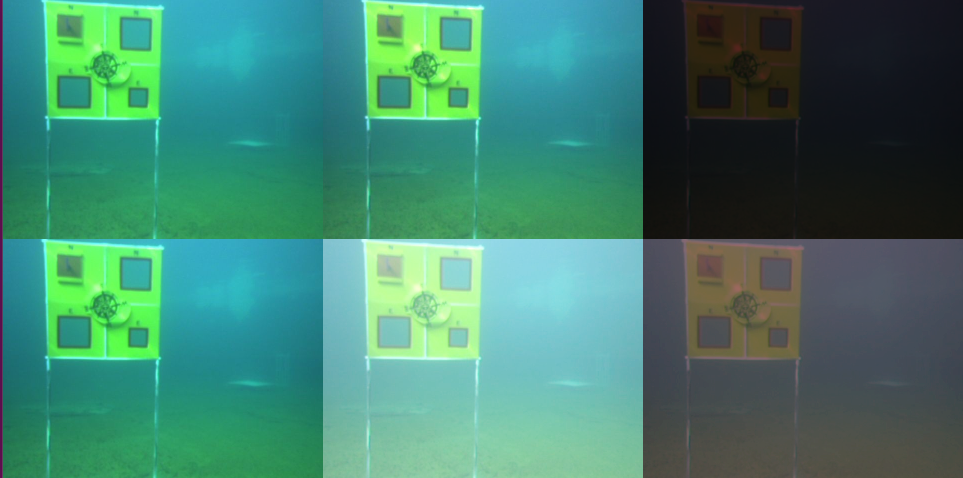
\includegraphics[width=0.8\textwidth, height=0.3\textheight]{color_gamma.png}
  \caption{Effect of applying gamma correction: (top row) no gamma correction,
    (bottom row) with gamma correction}
  \label{fig:color_gamma}
\end{figure}

To improve the result of color correction \outcite{cepeda2012combining}, gamma
correction is applied after color correction to illuminate dark areas in the
image (often effect of color normalization) which subsequently increase dynamic
range of the image.

\item \textbf{LAB color space} \\
Based on the evaluation of \outcite{kloss2009colour}, the CIE LAB color space
which reflects linearity of human colour perception is able to better represent
transformations for more subtle colours. Color normalization in LAB space will
rarely overcompensate or result in transformed image that looks unnatural.

\item \textbf{Grey pixel} \\

\begin{figure}[H]
\centering
  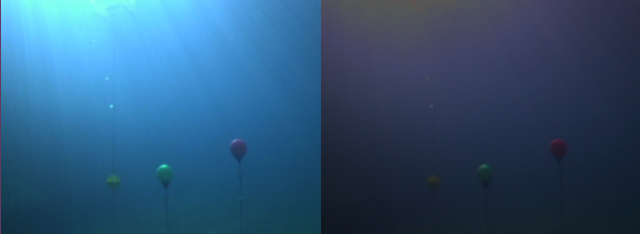
\includegraphics[width=0.7\textwidth, height=0.2\textheight]{greypixel.png}
  \caption{Applying novel grey pixel illumination estimation: a) Raw input, b)
    Color corrected}
  \label{fig:grey_pixel}
\end{figure}

\outcite{yang2015efficient} estimates the illuminant of the scene from
information of grey pixels detected in a color image. It assumes that
\textit{most of the natural images include some detectable pixels that are at
  least approximately grey}.Firstly, color image is converted to logarithm
space, followed by calculating the illumination-invariant measure (IIM) which is
calculated from local contrast of each logarithm channels. Then the mean of
selected grey pixels ranked by the Grey-Index will give us the estimated illumination.

\item \textbf{PCA based} \\

\begin{figure}[H]
\centering
  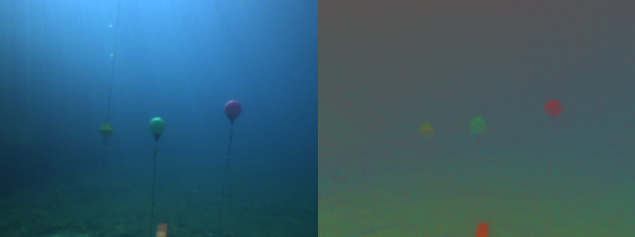
\includegraphics[width=0.7\textwidth, height=0.2\textheight]{spatialcolorconstancy.png}
  \caption{Spatial domain based illumination estimation: a) Raw input, b)
    Color corrected}
  \label{fig:spatial_colorconstancy}
\end{figure}
\end{enumerate}

The work of \outcite{cheng2014illuminant} estimates the illuminant by finding
bright pixels and dark pixels in a color image. The paper selects colours by
choosing n pixels with largest and smallest projected distance to the mean
vector. Then PCA is performed on the selected pixels to generate estimated
illumination direction.

\section{Underwater Image Enhancement}

Color normalization alone is insufficient to restore the original appearance of
an underwater obstacles. Underwater images also suffer from poor contrast,
overexposed or underexposed and flickering caused by refraction of sun light.

\begin{figure}[H]
\centering
  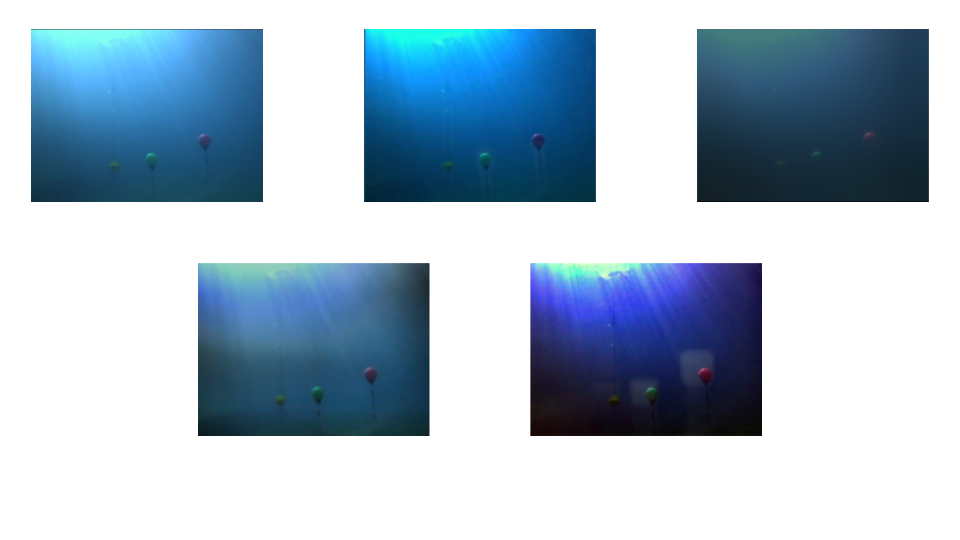
\includegraphics[width=0.8\textwidth, height=0.3\textheight]{enhancement_results.png}
  \caption{Underwater image enhancement results (left to right): \newline Top row:
  a) Raw input, b) Dark channel prior, c) Single image fusion \newline Bottom
  row: d) CLAHE, e) Red channel prior}
  \label{fig:underwater_image_enhancement_results}
\end{figure}

\subsection{Fusion-based image restoration}

\begin{figure}[H]
\centering
  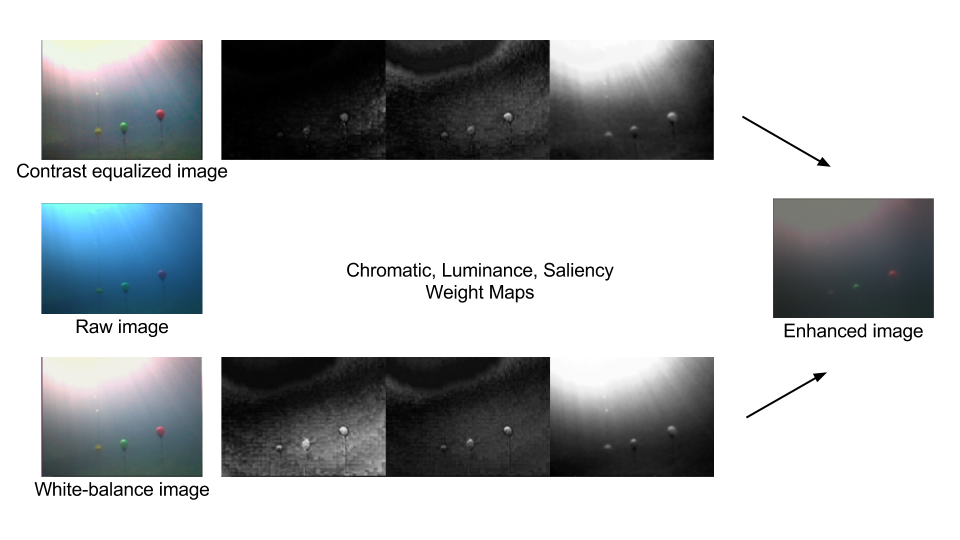
\includegraphics[width=0.8\textwidth, height=0.3\textheight]{fusion_pipeline.png}
  \caption{Single underwater image enhancement by fusion}
  \label{fig:fusion_pipeline}
\end{figure}

The work of \outcite{fang2013effective} suggests enhancement of underwater
images using a) white-balance image and b) contrast equalized image as inputs to
generate weight maps (chromatic, luminance, and saliency). The weight maps are
then normalized and fused using image pyramid approach to produce a smoother
enhanced image. The final output can be gamma corrected to adjust overall
brightness of the image.

\textbf{Chromatic map} controls the saturation gain of the enhanced image.
Higher saturation values yield more vivid color. \textbf{Luminance map} helps to
balance the brightness of the enhanced image while \textbf{Saliency map}
indicates area of high conspicuity. In other words, saliency map higlights area
that captures attention of the human visual system.

This approach has the added benefit of being extremely computationally fast and
simple to implement compared to other approach such as dark channel prior \outcite{he2011single}.

\subsection{Denoising \& Illumination Compensation}

According to the survey by \outcite{padmavathi2010comparison}, filters like
homomorphic filter, anisotropic filter and wavelet denoising filter are
necessary to suppress noise, preserve edge and smoothen underwater image. The
vision framework includes the following filters:

\begin{figure}[H]
\centering
  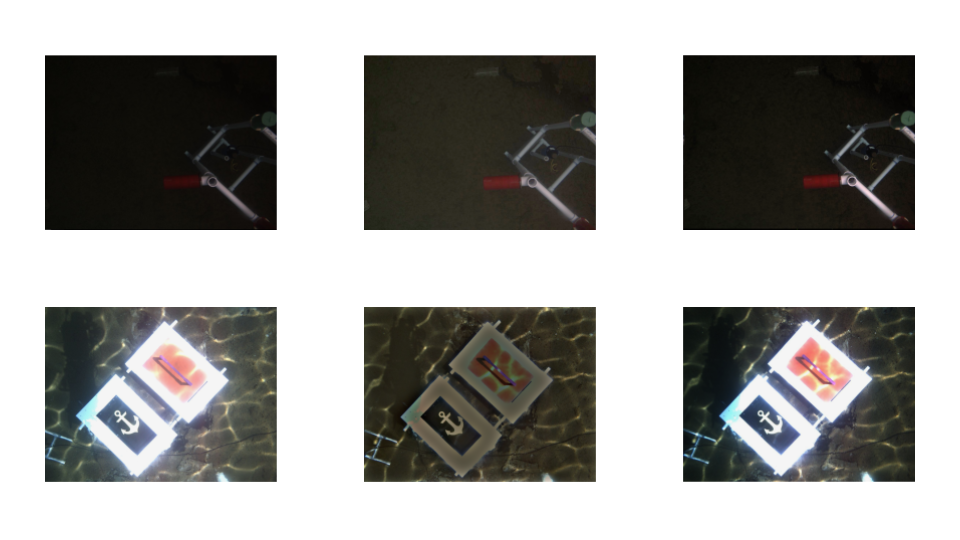
\includegraphics[width=0.8\textwidth, height=0.3\textheight]{illumination_compensation.png}
  \caption{Illumination compensation results (left to right): \newline Top row:
  a) Underexposed input, b) Chih's light compensation, c) Chen's light compensation \newline Bottom
  row: d) Flicker input, e) Homomorphic filter f) Gamma corrected}
  \label{fig:illumination_compensation_results}
\end{figure}

\begin{enumerate}

\item \textbf{Homomorphic filter} \\
Underwater vision tasks in shallow water are prone to suffer from spatial
temporal illumination patterns. In this case, a homomorphic filter can help to
correct non-uniform illumination and sharpen the image. With the assumption that
the high frequency components of an image is associated with reflectance of the
image, a high pass filter is applied on the frequency domain (removing
multiplicative noise) removing the low frequency (flickers).

\item \textbf{Anisotropic filter} \\
Use in conjuction with the homomorphic filter is the anisotropic filter which
smoothens homogeneous area while preserving edges. The work of
\outcite{perona1990scale} helps to reduce small edges generated by homomorphic filter.

\item \textbf{Illumination compensation} \\
When executing underwater vision tasks, the AUV has to constantly deal with
fluctuation in illumination because of various factors such as position of the
sun and clouds. Instead of relying on manual tuning of camera parameters, some
automated light compensation is performed on captured image sequence. This is
extremely important as an overexposed or underexposed image lose most of its
chromatic information.

\begin{figure}[H]
\centering
  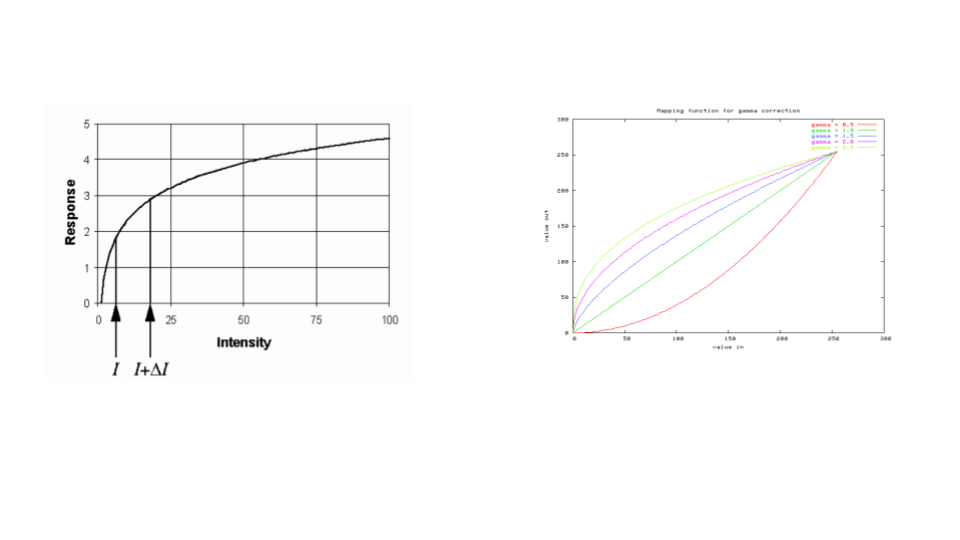
\includegraphics[width=0.8\textwidth, height=0.3\textheight]{lightcompensation.png}
  \caption{Comparison between logarithm curve and gamma curve}
  \label{fig:light_compensation}
\end{figure}

This paper refers to the work of \outcite{changlight} for 2 different
brightness adjustment algorithms. Firstly, a logarithm curve is used which obeys
the Weber-Fechner law of JND (Just noticeable difference) response instead of a
gamma curve which tends to enhance noise in dark regions.

\end{enumerate}

\section{Conclusion}

The preprocessing stage is one of the most important component for effective
underwater object tracking. Color normalization ensures repeatability of feature
extraction for different datasets. This allow for extracting domain invariant
features which can be used for object tracking in different water environments
such as public swimming pool, beach or a man-made lake (venue of Robosub competition).

However, it is necessary to keep the selection of preprocessing algorithms small
to reduce any overhead on real-time object tracking. Therefore, this paper
favors preprocessing algorithms that are less complex, effectively trading off
some degree of accuracy for lower detection latency.

%%%%%%%%%%%%%%%%%%%%%%%%%%%%%%%%%%%%%%%%%%%%%%%%%%%%%%%%%%%%%%%%%%%%%%%%%%%%%%%
% Chapter 5: Object Proposals
%%%%%%%%%%%%%%%%%%%%%%%%%%%%%%%%%%%%%%%%%%%%%%%%%%%%%%%%%%%%%%%%%%%%%%%%%%%%%%%

\chapter{Object Proposals}

Recently we have seen more state-of-the-art trackers incorpate object proposals
as part of their pipeline \outcite{Kristan2016a}, \outcite{kristan2015visual}.
The rise of object proposals which is a segmentation-based candidates generation
slowly replaces the more traditional sliding window approach which can be slow
when multiscale detection is required.

In addition, object proposals can be thought as a generic object detector which
generate candidate window based on some measure of objectness. Choosing the
criteria to measure the presence of an object is very important and is unique
for each domain of application. Object proposals according to
\outcite{hosang2016makes} fall into 2 large categories: a) grouping and b)
window ranking. 

\textbf{Grouping proposals} leverage on hierarchical segmentation approach to
generate overlapping segments with techniques such as a) superpixel grouping
(SP), b) solving multiple graph cut problem (GC) with random seeds or from c)
edge contour (EC). On the other hand, \textbf{Window scoring} proposals only
score each candidate window on likelihood of containing an object. This approach
is faster at the cost of lower localization accuracy.

From the mentioned paper, methods that are based on superpixel are not robust
towards illuminatin change while \textbf{BING} \outcite{cheng2014bing} and
\textbf{Edge-box} \outcite{zitnick2014edge} show promising result because of its
machine learning component (random forest).

\section{Algorithm Implementation}

\begin{figure}[H]
\centering
  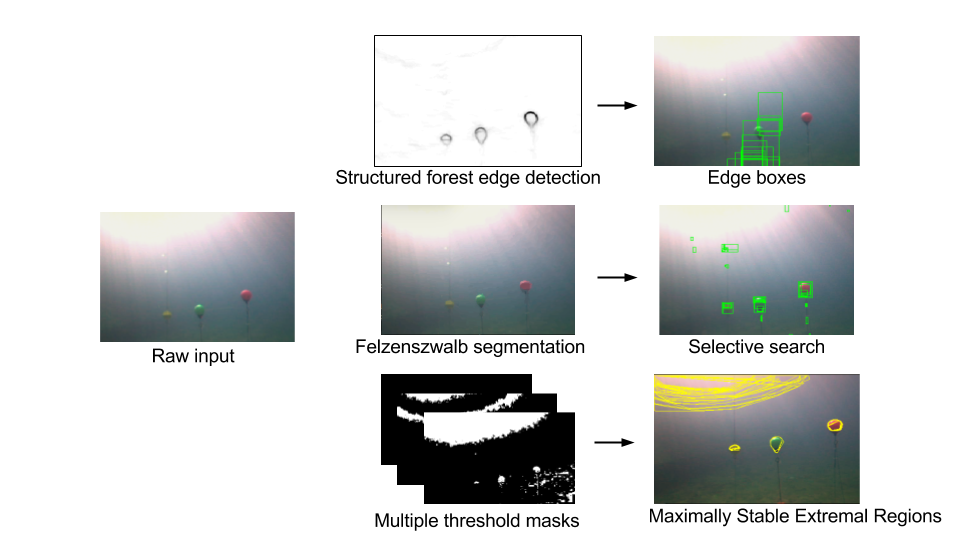
\includegraphics[width=0.8\textwidth, height=0.3\textheight]{proposals_results.png}
  \caption{Different object proposal paradigms}
  \label{fig:proposal_results}
\end{figure}

This paper utilizes 4 different object proposals for different type of
underwater vision tasks. Referring to Figure \ref{fig:proposal_results},
detection of color buoys which are largely homogeneous with little edge
information are much better handled with \textbf{SelectiveSearch}
\outcite{uijlings2013selective} approach. In general, \textit{grouping
  proposals} show more promising result than \textit{window scoring} approach
for all the underwater vision tasks. The additional speed gained from
\textit{window scoring} approach is almost nullified with the need to sample
large amount of windows to achieve decend localiztion accuracy.

Besides the \textit{SelectiveSearch} and \textit{Edge-box}, the following
section will discuss custom implementation of 2 other proposal methods.

\subsection{Maximially Stable Extremal Regions (MSER)}

\begin{figure}[H]
\centering
  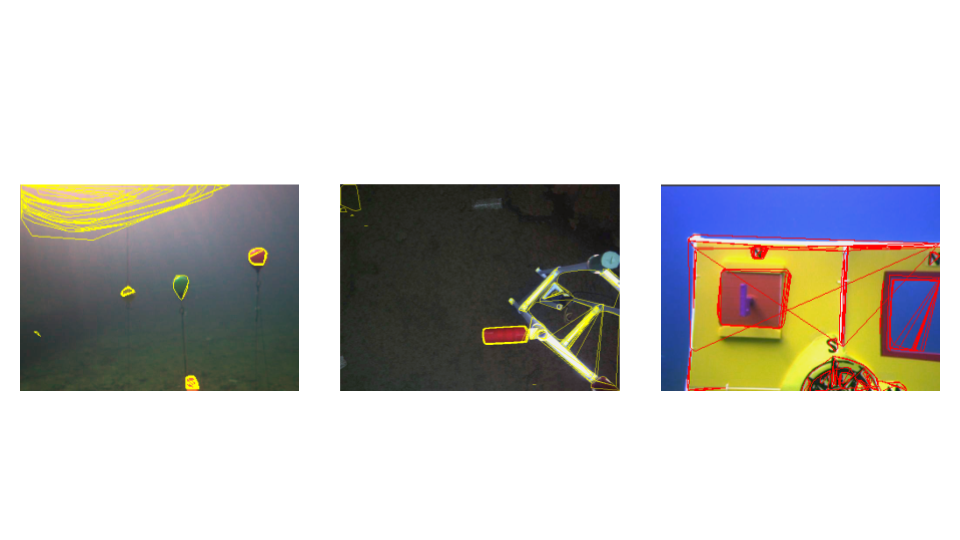
\includegraphics[width=0.8\textwidth, height=0.3\textheight]{mserproposal.png}
  \caption{Object proposals using MSER: a) Buoy task, b) Coin task, c) Set date task}
  \label{fig:mser_proposal}
\end{figure}

Since most the underwater obstacles are blob-like , this paper uses the
implementation of \outcite{forssen2007maximally} by OpenCV to extract candidate
windows for object detection. Firstly, the image is converted to HSV color
space. The \textit{Saturation} channel is then used for blob-detection as most
underwater obstacles have more vivid color compared to the background.
Alternatively, a combination of different color channels are explored to
generate more segments such as L*a*b and YUV.

\subsection{Saliency-based}

Object proposals based on salient cues are also explored as they mimic closely
how human visual system works. Without any preprocessing, the results of salient
object proposal is mediocre at best compared to the other proposal methods.
However with appropriate color normalization and enhancement, this method can
produce results that can rival with \textit{SelectiveSearch} and
\textit{Edge-box} in this domain of application. This paper use an open-source implementation of:

\begin{figure}[H]
\centering
  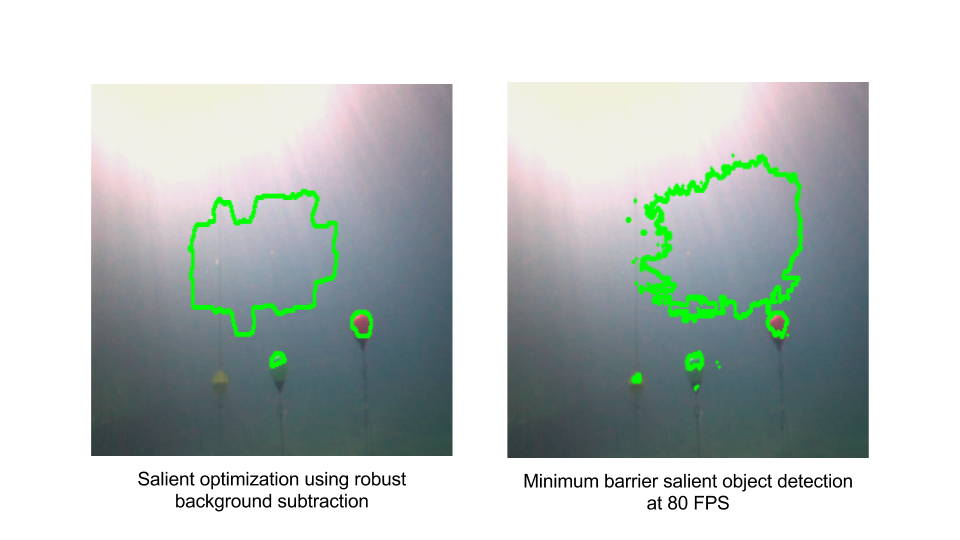
\includegraphics[width=0.8\textwidth, height=0.3\textheight]{saliency.png}
  \caption{Object proposals using saliency approach}
  \label{fig:salient_proposal}
\end{figure}

\begin{enumerate}
  \item \textbf{Saliency optimization from robust background subtraction} \outcite{zhu2014saliency}
  \item \textbf{Minimum Barrier Salient Object Detection at 80 FPS} \outcite{zhang2015minimum}
  \item \textbf{Frequency-tuned Salient Region Detection} \outcite{achanta2009frequency}
\end{enumerate}

\section{Conclusion}

In this section we have explored different proposal methods that are
state-of-the-art and others (MSER and saliency) that are slightly different from
available literatures. Though \textit{MSER} managed to generate a lot of
segments, this method does not measure the quality of each segment unlike
\textit{Edge-box}. \textit{Salient object proposals} on the hand produce
candidate windows that are highly accuracte but with very few segments. In
general, not missing any possible object candidate is more important than
generating highly accurate candidate window. Therefore, this paper propose to
lower the threshold for \textit{saliency-based} proposals in order to generate
more candidate windows.

%%%%%%%%%%%%%%%%%%%%%%%%%%%%%%%%%%%%%%%%%%%%%%%%%%%%%%%%%%%%%%%%%%%%%%%%%%%%%%%
% Chapter 7: Feature Design
%%%%%%%%%%%%%%%%%%%%%%%%%%%%%%%%%%%%%%%%%%%%%%%%%%%%%%%%%%%%%%%%%%%%%%%%%%%%%%%

\chapter{Feature Design}

Large amount of feature detector and descriptors used for this projects are available in
\href{http://opencv.org/}{OpenCV} or
\href{http://scikit-image.org/}{Scikit-image}. This paper has come to this list
of features based on the benchmarks by \outcite{lee2016recent} and \outcite{pieropan2016feature}.
Below is a summary of features available in this vision framework:

\begin{enumerate}
  \item \textbf{SURF} \outcite{bay2006surf}
  \item \textbf{SIFT} \outcite{lowe1999object}
  \item \textbf{BRISK} \outcite{leutenegger2011brisk}
  \item \textbf{ORB} \outcite{rublee2011orb}
  \item \textbf{FREAK} \outcite{alahi2012freak}
  \item \textbf{MSER} \outcite{forssen2007maximally}
  \item \textbf{DAISY} \outcite{tola2010daisy}
  \item \textbf{CenSure} \outcite{agrawal2008censure}
  \item \textbf{LBP} \outcite{ojala2002multiresolution}
  \item \textbf{AKAZE} \outcite{alcantarilla2011fast}
  \item \textbf{Inner Shape Context} \outcite{ling2007shape}
  \item \textbf{Elliptic Fourier Feature of Closed Contour} \outcite{kuhl1982elliptic}
  \item \textbf{Histogram of Oriented Gradient} \outcite{dalal2005histograms}
  \item \textbf{Hu moment and Zernike moment} \outcite{sabhara2013comparative}
\end{enumerate}

\section{Requirements}

There are various desired properties of features for underwater object tracking
in particular ones that are highly applicable in the competition setting of
Robosub competition.The 2 main properties are: a) \textit{repeatability} and b)
\textit{discriminability}. Firstly, it is important that we are able to
consistently extract the same set of features for the same object in order to
achieve consistent detection. However, there is always a trade-off with
\textit{discriminability} as features that are highly repeatable tend to
describe a more general representation of the object.

\subsection{Illumination invariance}

It is preferable to have features that are highly invariant to sudden changes in
illumination as the operational depth of the AUV during the competition is still
susceptible to external factors such as position of the sun and clouds.To
achieve this, this paper propose usafe of multiple illumination invariation
color space to describe appearance of the object.

\subsection{Scale \& Rotation invariance}
Secondly, the feature must also be scale and rotation invariant because the AUV
will be constantly navigating around its surrounding to identify object of
interest. The easies way to achieve this is to rely on purely color-based
feature that will be mentioned in section \ref{sec:color_descriptors}. Color-based features are easier to
compute and are less computationally expensive compared to features like SURF,
SIFT and HOG.

\subsection{Shape discriminability}

\begin{figure}[H]
\centering
  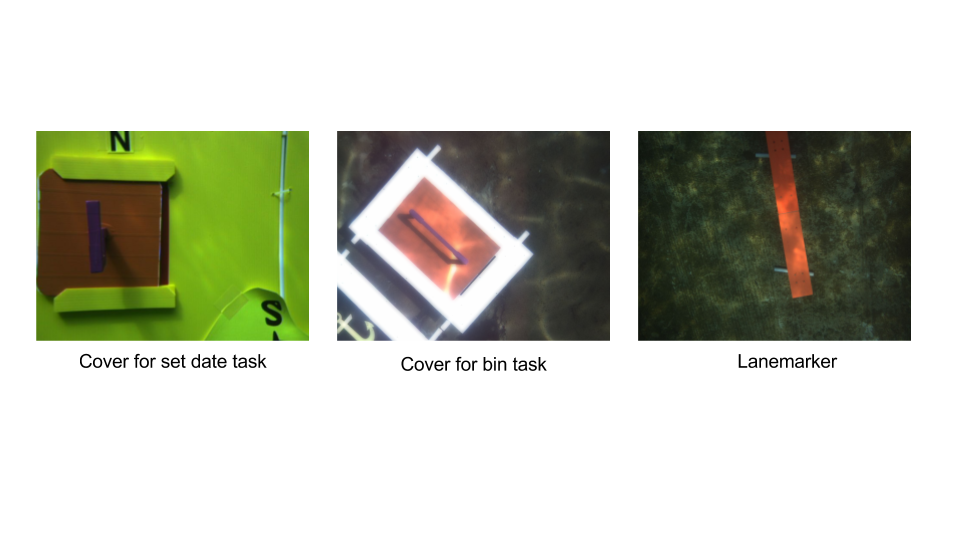
\includegraphics[width=0.8\textwidth, height=0.3\textheight]{similarcolor.png}
  \caption{Objects with similar colors}
  \label{fig:similar_color}
\end{figure}

Color-based features alone are not sufficient for our application as there
exists objects of similar color appearance. In this case, we will need shape
descriptors that will be elaborated in section \ref{sec:shape_descriptors}.

\section{Color space: Implementation}
\label{sec:color_descriptors}

Besides the usual color spaces, this section will look at some implementation
of color spaces based on these papers on the subject:

\begin{enumerate}

  \item Detecting salient cue through color-ratio \outcite{todt2004detecting}
  \item Color Invariants for Person Re-identification \outcite{kviatkovsky2013color}
  \item Evaluation of Color Descriptors for Object and Scene Recognition \outcite{van2010evaluating}
  \item Invariant color descriptors for efficient object recognition \outcite{sande2011invariant}
  \item A Perception-based Color Space for Illumination-invariant Image
    Processing \outcite{chong2008perception}
  \item Illumination invariant color model robot soccer \outcite{luan2010illumination}
  \item Illumination invariant imaging \outcite{maddern2014illumination}
  \item Color Model Double Opponency \outcite{gao2013color}

\end{enumerate}

\subsection{rg chromacity}

\[
  r = \frac{R}{R + G + B}, g = \frac{G}{R + G + B}, b = \frac{B}{R + G + B}
\]

\subsection{Normalized RGB}

\[
  r = \frac{R - \mu(R)}{\sigma(R)}, g = \frac{G - \mu(G)}{\sigma(G)}, b =
  \frac{B - \mu(B)}{\sigma(B)}
\]

\subsection{Opponent color space}

\[
\begin{aligned}
  O1 = \frac{R - G}{\sqrt{2}}, O2 = \frac{R + G - 2B}{\sqrt{6}}, O3 = \frac{R +
    G + B}{\sqrt{3}} \\
  W_{o1} = \frac{O1}{O3}, W_{o2} = \frac{O2}{O3}
\end{aligned}
\]

\subsection{Log color ratio}

\[
  L1 = \log{\frac{R}{B}}, L2 = \log{\frac{R}{B}}, L3 = \log{\frac{G}{B}}
\]

\subsection{RGBY opponent space}

\[
  R_o = R - \frac{G + B}{2}, G_o = G - \frac{R + B}{2}, B_o = B - \frac{R +
    G}{2}, Y_o = \frac{R + G}{2} - \abs{R - G} - B
\]

\subsection{DCD: Dominant color descriptor}

Convert to LUV color space or any other perceptually unifrom color space.
Perform K-mean clustering and return the percentage of pixels and variance of
each color centers.

\section{Shape descriptors}
\label{sec:shape_descriptors}

\subsection{Inner shape context}

\begin{figure}[H]
\centering
  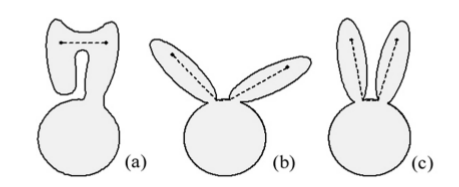
\includegraphics[width=0.5\textwidth, height=0.1\textheight]{innerdistance.png}
  \caption{Dashed lines denote shortest path withint the shape boundary}
  \label{fig:inner_shapecontext}
\end{figure}

\textit{Inner-distance} is defined as the length of the shortest path between
landmark points within the shape silhouette. Inner distance is used instead of
Euclidean distance when building the shape context. This is an improvement over
the traditional shape context as it is able to describe more complicated shapes.

\subsection{Elliptic Fourier Feature of Closed Contour}

A chain-encoded closed contour is first obtained using OpenCV's
\textit{findContour}. Normalization of Fourier's coefficients using various
elliptical properties of the coefficients. This descriptors obtained are
invariant to \textit{rotation}, \textit{dilation} and \textit{translation} of
the contour.

\subsection{Moment-based descriptors}

The vision framework includes 2 common moment-based descriptors: a) \textit{Hu Moment}
and b) \textit{Zernike Moment}. According to the evaluation by
\outcite{sabhara2013comparative}, Zernike's moment is more robust and flexible
as one can varies the order of polynomial to describe more complex shape.
Furthermore, the Pseudo-Zernike's moment which more robust to noise is also part
of the supported shape descriptors.

In addition, simpler contour properties can also be used if the target of
interests consist of basic shapes that are largley different from each other.
These properties include:

\begin{enumerate}

  \item \textbf{Eccentricity} \\
  Fit a bounding box over the closed contour to obtain the lenght of major axis
  and length of the minor axis.

  \[
    Eccentricity = \frac{L_{major axis}}{L_{minor axis}}
  \]

  \item \textbf{Circularity ratio} \\
  Calculates the ratio between the area of original shape and area of its enclosing circle.

  \[
    Circularity = \frac{Area_{shape}}{Area_{circle}}
  \]

  \item \textbf{Rectangularity} \\
  Similar to above, this calculates the ratio between area of the original shape
  and area of its enclosing rectangle.

  \[
    Rectangularity = \frac{Area_{shape}}{Area_{rectangle}}
  \]

\end{enumerate}

%%%%%%%%%%%%%%%%%%%%%%%%%%%%%%%%%%%%%%%%%%%%%%%%%%%%%%%%%%%%%%%%%%%%%%%%%%%%%%%
% Chapter 8: Model Learning
%%%%%%%%%%%%%%%%%%%%%%%%%%%%%%%%%%%%%%%%%%%%%%%%%%%%%%%%%%%%%%%%%%%%%%%%%%%%%%%

\chapter{Model Learning}

The primary classifiers for object classification include: a) \textit{SVM}, b)
\textit{Random Forest}, and \textit{Gaussian Process}. These classifiers are
selected primarily because we have small amount of data as availability of
undewater data are quite limited and can be very expensive to collect. Neural
network and its more popular sibling: Deep Neural Network is largely ignored
because of a) scarcity of data and b) many parameters tuning are needed. In
addition,  this vision framework hopes to achieve comparable accuracy in
underwater object tracking relying more simple features and less parameters
intensive tuning from human experts.

\begin{figure}[H]
\centering
  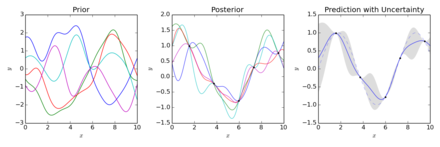
\includegraphics[width=0.5\textwidth, height=0.1\textheight]{gp.png}
  \caption{Gaussian process}
  \label{fig:gp}
\end{figure}

\textit{Gaussian process (GP)} \outcite{rasmussen2006gaussian} is introduced
because of its unique ability to perform feature selection using a covariance
function that implements \textit{automatic relevance determination}. A GP model
also provides uncertainty scores of each classification and a prior knowledge
can be integrated easily into its prior function. One major downside of GP is
definitely its $O(n^3)$ complexity which makes it a poor choice for large amount
of data.

The following section will focus more on the effort to apply the
\textit{automatic machine learning} principle which aims to automate trivial
machine learning tasks such as \textit{feature selection}, \textit{model
  selection} and \textit{hyperparameters optimization}. Most of these algorithms
are open-source and are readily available, this paper merely tries to integrate it
as part of the framework to remove the dependency on machine learning experts
for trivial tasks.

\section{Feature Selection}

Having multiple features is advantageous to allow for greater adaptation to
different challenging environments. For instance, detection of a textureless
object can be challenging using the popular HOG feature while a simple color
histogram can produce a better result. This paper would like to highlight that
choosing the right feature can improve accuracy and reduce needless
computational cost from using complex feature descriptors like SIFT. In
addition, choosing best features also reduce dimension of feature which is a
problem on small AUV equipped with less powerful computing unit.

Besides using the \textit{Automatic relevance determination} of a GP model, this
framework leverages on the widely used machine learning library,
\textit{Sklearn's feature selection module}. Below is the list of feature
selection functions used in the vision framework.

\begin{enumerate}

    \item \textbf{Removing feature with low variance} \\
    This approach removes features that are below certain variance threshold
    labelling it as redundant.

    \item \textbf{Univariate feature selection}
    Univariate test such as F-test and chi-test are used to select the best
    features before training the model.

    \item \textbf{Tree-based}
    Uses an ensemble model (forest of trees) to calculate feature importances
    which is used to score input features.

\end{enumerate}

\section{Hyperparameters optimization: Implemetation}

Uses \href{https://github.com/automl/HPOlib}{HPOlib} which contains 3 libraries for hyperparameter optimizations:

\begin{enumerate}
  \item Sequential model-based optimization \outcite{hutter2011sequential}
  \item Spearmint Bayesian optimization codebase \outcite{snoek2012practical},
    \outcite{swersky2013multi}, \outcite{snoek2014input},
    \outcite{snoek2013bayesian}, \outcite{gelbart2014bayesian}
  \item Hyperopt
\end{enumerate}

Ideally, there are very few hyperparameters optimization needed as the paper
actively tries to use non-parametric methods with the exception of SVM (choice
of kernel and misclassificatin penalty).

\section{Model Selection}

For model selection, again \textit{Sklearn's model selection and evaluation} is
used to select the best model for a particular tasks through cross-validation.
From our observation, the performance of each classifiers does not varies very
much. In addition, this paper also experimented with \textit{Auto sklearn}
\outcite{feurer2015efficient}. 

%%%%%%%%%%%%%%%%%%%%%%%%%%%%%%%%%%%%%%%%%%%%%%%%%%%%%%%%%%%%%%%%%%%%%%%%%%%%%%%
% Chapter 9: Object Tracking
%%%%%%%%%%%%%%%%%%%%%%%%%%%%%%%%%%%%%%%%%%%%%%%%%%%%%%%%%%%%%%%%%%%%%%%%%%%%%%%

\chapter{Object Tracking}

This section will explore different tracking paradigm
\outcite{stalder2012paradigms} and analyze various surveys conducted to determine the best trackers
for underwater visual tracking. Because of the tracking strategy, only single
object tracking algorithms are evaluated. There are few reasons why the paper
proposed a single object tracking approach:

\begin{enumerate}
  \item Simpler implementation
  \item The AUV has limited number of manipulators which make it possible of
    manipulating only a single obstacle at a time
  \item Less computationally expensive
\end{enumerate}

\section{Benchmarks}

As for the benchmarks, the paper looks into the papers listed below:

\begin{enumerate}
  \item Visual object tracking performance measures revisited \outcite{Cehovin2016a}
  \item VOT 2016 Challenge Results \outcite{Kristan2016a}
  \item VOT 2015 Challenge Results \outcite{kristan2015visual}
  \item Is my new tracker really better than yours ? \outcite{Cehovin2014a}
\end{enumerate}

The top trackers almost always combine an adaptive tracking and a fixed-model
tracking approach. Online model update techniques such as \textit{Adaboost} and
\textit{Multiple Instance Learning} are capable of adapting to different
conditions as positive samples are sampled around vicinity of tracked object
while negative samples are extracted from background of the image. However,
adaptive model update comes at the cost of computational cycle and also more
complicated model. 

\section{Tracking by detection: Implementation}

\begin{figure}[H]
\centering
  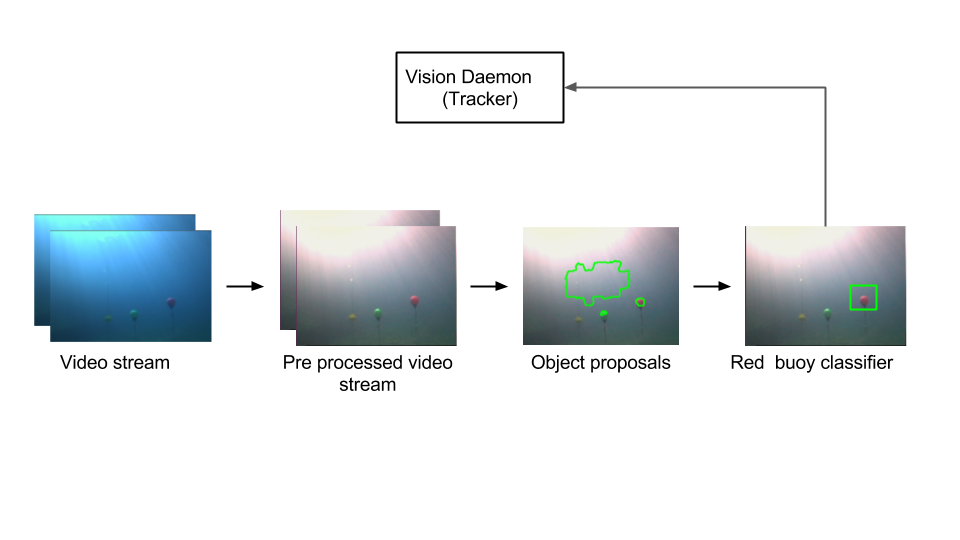
\includegraphics[width=0.8\textwidth, height=0.3\textheight]{tracker.png}
  \caption{Tracking pipeline}
  \label{fig:tracker}
\end{figure}

This paper utilizes a tracking by detection approach as detection is performed
on each frame and associated with previously tracked objects. A tracker is
\textbf{terminated} when an the tracker loses track of its target for at least
10 frames. This value is determined through empirical evaluation of applying the
tracker on existing image sequence. To handle \textbf{multiple instance} of the
object, the object with the shortest Euclidean distance will be selected. In
addition, association of object with previously tracked object is bounded on a
specific radius to reduce false positives with the assumption that the AUV is
perfectly stable and does not move randomly over a short period of time.

Prior knowledge such as geometric property of the target can be included through
a weighted summation of classification score and prior score. With more context,
a more accurate detection can be achieved.

\section{Model-free tracking: Implementation}

In addition to the main tracking strategy mentioned above, model-free tracking algorithms
based on correlation-filter are also included for: a) rapid data collection and
b) tracking generic object. These algorithms include:

\begin{enumerate}
  \item High-speed kernelized correlation filter \outcite{henriques2015high}
  \item Visual Object Tracking using Adaptive Correlation Filters \outcite{Bolme2010}
\end{enumerate}

%%%%%%%%%%%%%%%%%%%%%%%%%%%%%%%%%%%%%%%%%%%%%%%%%%%%%%%%%%%%%%%%%%%%%%%%%%%%%%%
% Chapter 10: Experimental results
%%%%%%%%%%%%%%%%%%%%%%%%%%%%%%%%%%%%%%%%%%%%%%%%%%%%%%%%%%%%%%%%%%%%%%%%%%%%%%%

\chapter{Experimental results}

\section{Datasets}

The datasets are generated and categorized using the sequence annotator, AIBU
which is used by the Visual Object Tracking (VOT) committee. There are total of
6 datasets with different set of challenges. At the same time, 6 object classes
will be tested.

\subsection{Challenges}

Figure \ref{fig:dataset1} and \ref{fig:dataset2} are the datasets labelled with
bounding box ground truth used for evaluation of the proposed tracker.

\begin{figure}[H]
\centering
  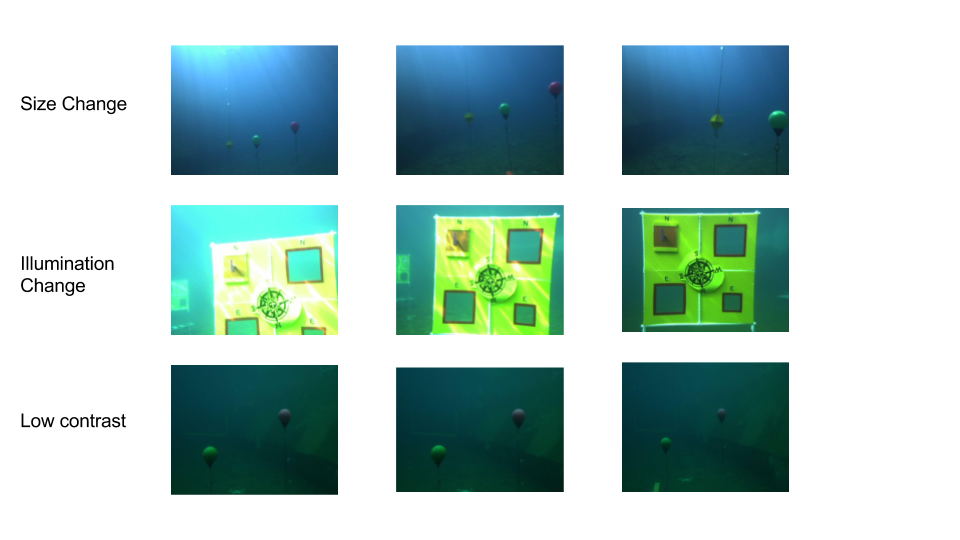
\includegraphics[width=0.8\textwidth, height=0.3\textheight]{data1.png}
  \caption{Dataset 1}
  \label{fig:dataset1}
\end{figure}

\begin{figure}[H]
\centering
  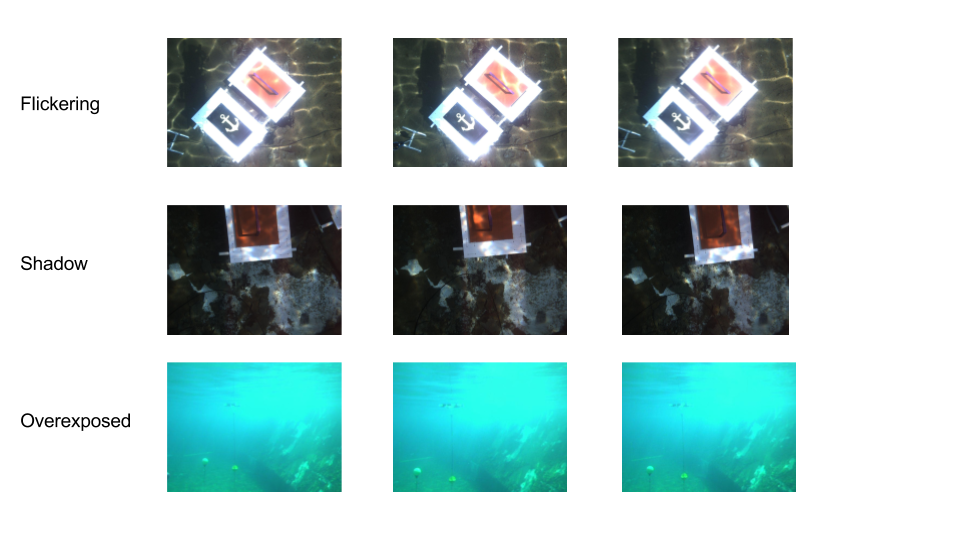
\includegraphics[width=0.8\textwidth, height=0.3\textheight]{data2.png}
  \caption{Dataset 2}
  \label{fig:dataset2}
\end{figure}

\subsection{Object classes}

The objects to be tracked composed of:

\begin{enumerate}
  \item Red buoy
  \item Green buoy
  \item Yellow buoy
  \item Set date cover
  \item Red Coin
  \item Bin cover
\end{enumerate}

\section{Results}

\subsection{Evaluation methodology}

Using Visual Object Tracking (VOT15) \outcite{kristan2015visual} as guideline,
following are the performance measures used:

\begin{enumerate}

  \item \textbf{Accuracy, A} \\
  Accuracy is measured the average overlap of predicted bounding box with the
  ground truth bounding box. Accuracy for a sequence is obtained by averaging
  per-frame accuracies.
  
  \item \textbf{Robustness, R} \\
  Robustness measures how many times the tracker loses the target (overlap is
  zero). The tracker is reinitialized 10 frames after the failure. Again,
  robustness of a sequence is calculated using the average failure rate.

  \item \textbf{Frame per-second, FPS}
  This is a naive measure of speed by calculating the average of FPS of the
  tracker over different datasets.

\end{enumerate}

\subsection{Trackers}

The competing trackers can be categorized into 2 big categories: a) variations
of proposed tracker and b) open-source trackers. The baseline tracker is our
proposed tracker without any preprocessing, using only color thresholding along
with contour properties. Below is the list of trackers:

\begin{table}[H]
\centering
\begin{tabular}{|l|}
\hline
Trackers                           \\ \hline
Baseline                           \\ \hline
Baseline + preprocessing           \\ \hline
Baseline + preprocessing +  automl \\ \hline
MOSSE                              \\ \hline
KCF                                \\ \hline
EBT (Edge Box Tracker)             \\ \hline
\end{tabular}
\caption{Competing trackers}
\label{table:competing_trackers}
\end{table}

It is to be made known that only minimal preprocessing such as smoothing and
denoising are performed when using open-source trackers. This is to ensure that
the inputs are not too perturbed with noise. This makes sure that the
state-of-the-art trackers are not at a big disadvantage compared to our proposed trackers. 

\subsection{Raw results}

\begin{table}[H]
\centering
\begin{tabular}{|l|l|l|l|}
\hline
Trackers                           & Accuracy & Robustness & Speed \\ \hline
Baseline                           & 0.21     & 7.23       & 200   \\ \hline
Baseline + preprocessing           & 0.34     & 6.11       & 50    \\ \hline
Baseline + preprocessing +  automl & 0.53     & 2.53       & 50    \\ \hline
MOSSE                              & 0.30     & 8.10       & 100   \\ \hline
KCF                                & 0.35     & 4.91       & 70    \\ \hline
EBT (Edge Box Tracker)             & 0.41     & 3.11       & 43    \\ \hline
\end{tabular}
\caption{Raw results across all datasets}
\label{table:raw_results}
\end{table}

\section{Discussion}
  
\subsection{Preprocessing}

Both correlation filter based trackers, KCF and MOSSE performed poorly for the
\textit{illumination-dataset} while our proposed tracker managed to consistently
track the object of interest. EBT on the other hand showed poor performance in
both \textit{overexposed} and \textit{low contrast} datasets as the edge
information is barely visible. For the \textit{size change} dataset, KCF and EBT in
particular shows the best performance. This is to be expected as these trackers
did show promosing result in VOT15. The baseline tracker without any
preprocessing performed miserably in almost all datasets. However, with added
preprocessing, the basline tracker is able to achieve decent accuracies for
datasets without any complex shapes.

\subsection{Automatic machine learning}

The result for performing feature selection showed promising result as it is
able to perform up to par with some of the state of the art trackers such as EBT
and KCF. However, it has to be mentioned that these trackers with preprocessing
are able to outperform the proposed tracker. This goes to show the importance of
preprocessing when performing object detection in underwater environment.

\subsection{Conclusion}

Looking at the Table \ref{table:raw_results}, one can conclude the importance of
preprocessing for underwater object tracking because the accuracies achieved by
state-of-the-art trackers do not justify their ranking in VOT15. Our proposed
tracker which combines both preprocessing and automatic machine learning
approach is able improve the baseline accuracies by leaps and bounds without
needing to really complex feature representations.

\bibliographystyle{socreport}
\bibliography{fyp}{}

%%% End document
\end{document}
